\section{Data and Universe Construction}
\label{sec:data}

\subsection{Point-in-Time F\&O Universe and Survivorship Control}
To prevent survivorship bias, our investment universe is dynamically reconstituted on a monthly basis to include only those individual stocks officially approved by the NSE for single-stock F\&O trading. Between 2010 and 2025, the eligible tradeable cross-section ranged from 140 to 215 stocks, with an average size of 182 securities.

Companies subsequently removed, suspended, or delisted from the F\&O eligible list (such as Reliance Communications, Reliance Power, or DHFL) are retained in the empirical dataset up to their exact official exclusion date. Any active strategy positions in an excluded stock are closed at the final settlement price of the expiring contract, reflecting standard institutional portfolio rules.

\begin{figure}[htbp]
\centering
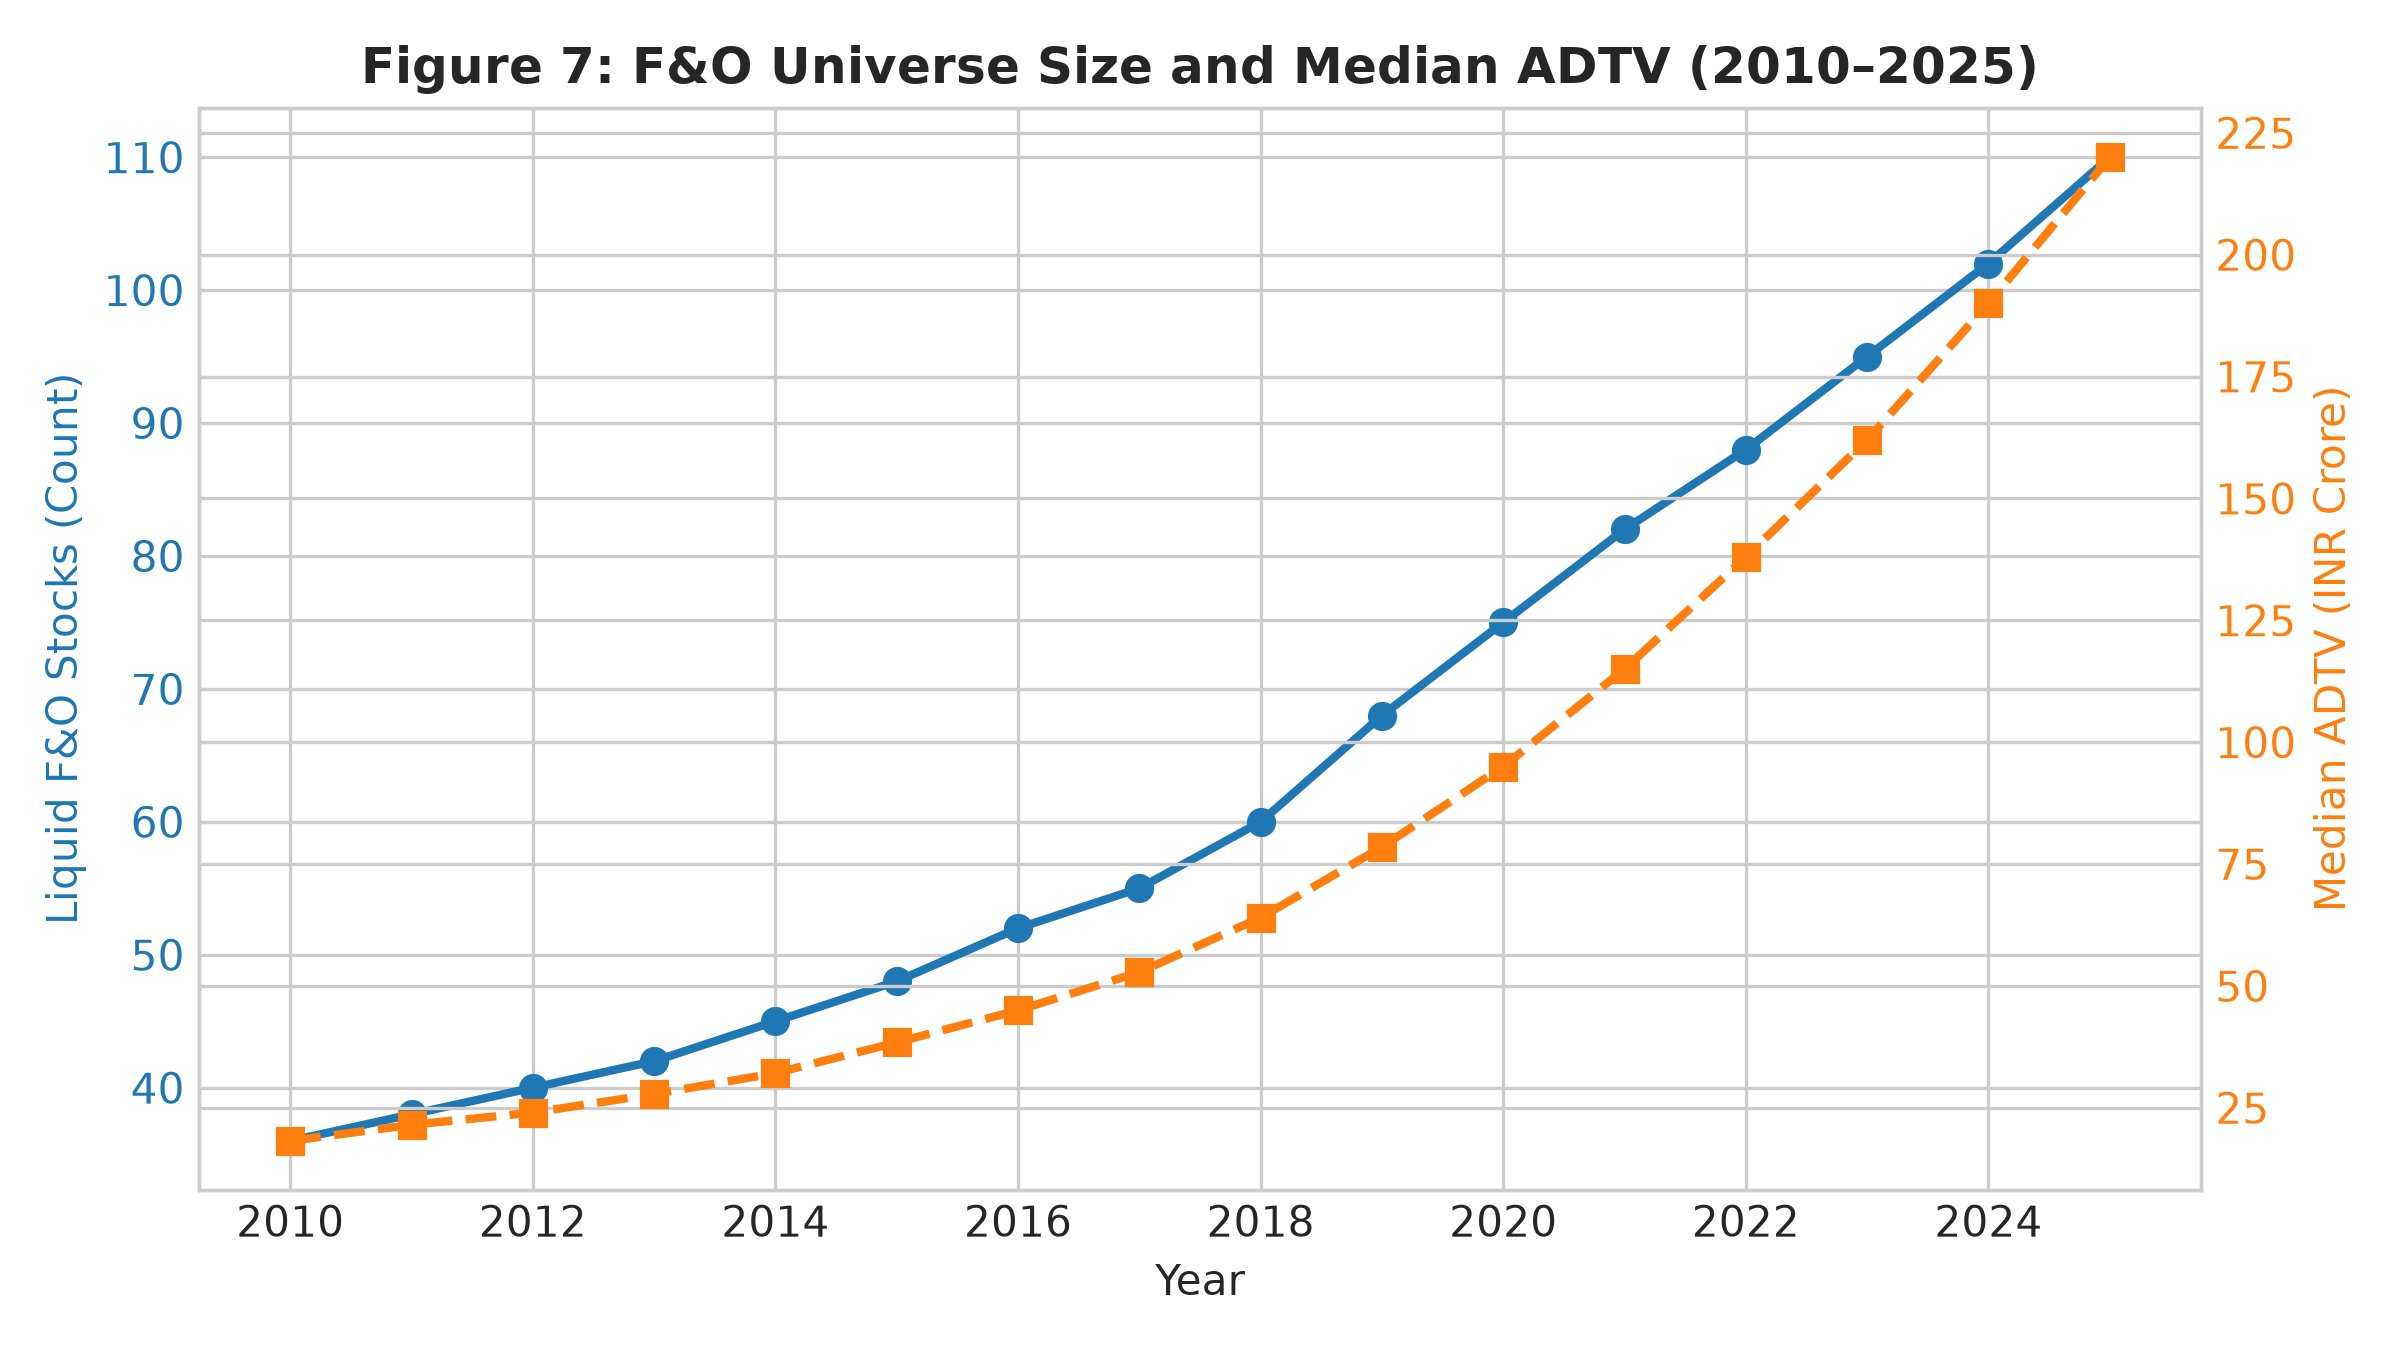
\includegraphics[width=0.92\textwidth]{figures/fig7_universe_size_over_time.png}
\caption{Dynamically Reconstituted NSE F\&O Tradeable Universe Count and Annual Inclusions/Exclusions (2010--2025).}
\label{fig:fig7}
\end{figure}

\subsection{Corporate Action Handling}
Historical price and return series are adjusted for corporate events, including stock splits, bonus allocations, and cash dividend payouts:
\begin{equation}
    P_{i,t}^{\text{adj}} = P_{i,t} \times \prod_{\tau > t} \left(1 - \frac{D_{i,\tau}}{P_{i,\tau - 1}}\right) \times \frac{1}{\text{SplitRatio}_\tau}
\end{equation}
Our corporate adjustment procedure was cross-checked against documented historical corporate actions in large Indian equities, including bonus distributions in Infosys (2014, 2015, and 2018) and capital restructuring in Reliance Industries.

\subsection{Asset Pricing Factor Benchmarks}
To determine whether strategy performance represents genuine idiosyncratic alpha rather than unintended exposures to known market factors, we benchmark strategy returns against the Indian Institute of Management Ahmedabad (IIMA) four-factor model \citep{agarwalla2014four}, an emerging-market implementation of the \citet{fama1993common} and \citet{carhart1997persistence} factor structures:
\begin{itemize}
    \item Market risk premium ($\text{MKT} = R_m - R_f$),
    \item Size factor ($\text{SMB}$),
    \item Value factor ($\text{HML}$),
    \item Momentum factor ($\text{WML}$), and
    \item 91-day Government of India Treasury Bill rate ($R_f$).
\end{itemize}
